\chapter{Výsledky a diskusia}

\section{Vývoj publikačnej činnosti a citovanosti pracovníkov celej Fakulty
  prírodných vied v~čase}

Obrázok~\ref{fig:plot.fns.publications} vyjadruje grafické znázornenie množstvo
publikovaných článkov všetkými pracovníkmi Fakulty prírodných vied
v~jednotlivých rokoch z~citačných registrov Scopus a WoS (samostatné krivky).  Je
prirodzené, že pracovníci slovenskej univerzity viac článkov publikujú
v~európskych časopisoch, pre ktoré má Scopus väčšie pokrytie než WoS.  Čo môžeme
vidieť ako rozdiel kriviek v~období 2004--2010.  Publikačný skok WoS od roku
2012 je spôsobený obsiahnutím šesťnástich kapitol z~knihy \emph{Handbook of
  Magentochemical Formulae} od doc.\,Boču z~Katedry chémie, ktoré nie sú
citované (knihy sú o~mnoho menej citované ako vedecké články).  Zvýšenie počtu
publikácií vo WoS v~roku 2015 je dôsledkom tlaku na získanie akreditácie.  Pre
akreditačná komisiu komisiu sú najdôležitejšie časopisy indexované vo WoS.

\begin{figure}
  \centering
  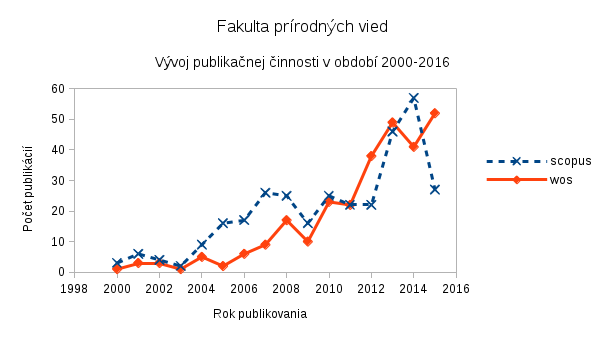
\includegraphics[width=\textwidth]{obr/plot-fns-publications.png}
  \caption{Vývoj publikačnej činnosti pracovníkov FPV UCM v~období 2000--2016.}
  \label{fig:plot.fns.publications}
\end{figure}

Graf na obrázku~\ref{fig:plot.fns.citations} zobrazuje celkový počet citácií
článkov publikovaných v~danom roku.  Rozdiel v~citáciách medzi dátami z~Scopusu
a WoS sú viditeľné hlavne už spomínanom období 2004--2010.  Extrémny rozdiel
citácií na publikácie z~roku 2005 je spôsobený, že v~citačnom registri Scopus je
obsiahnutých 16 článkov z~roku 2005, ktorých 15 sú dobre citované.  WoS obsahuje
iba dva články z~tohto roku: ten necitovaný zo Scopusu a publikáciu, ktorá je
obsiahnutá iba v~databáze z~WoS, ale tiež bez citácií.  Zvýšenie počtu
publikáciách v~časopisoch indexovaných WoS neznamená vyššiu kvalitu článkou čo
vidíme počte citácií pre rok 2015.

\begin{figure}
  \centering
  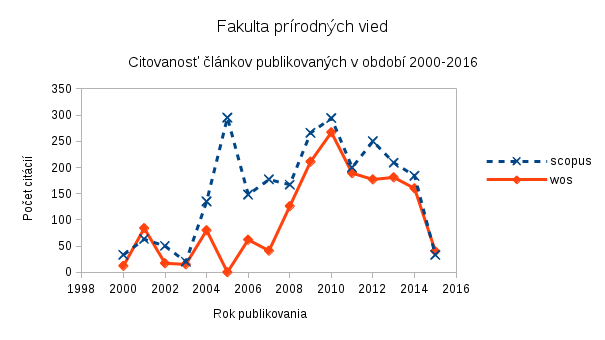
\includegraphics[width=\textwidth]{obr/plot-fns-citations.png}
  \caption{Citovanosť článkov všetkých pracovníkov FPV UCM za obdobie 2000--2016.}
  \label{fig:plot.fns.citations}
\end{figure}



\section{Vývoj publikačnej činnosti a citovanosti pracovníkov Katedry biológie
v~čase}

Na obrázku~\ref{fig:plot.bio.publications} je zobrazený počet článkov
publikovaných každým rokom v~období 2000--2016.  Vzostup publikácií vo WoS pre
rok 2013 je spôsobený už spomínanou akreditáciou.  Dáta zo Scopusu obsahujú tri
články naviac oproti dátam z~WoS.  Najväčší počet publikácií má doc.\,Janeček
(17 v~Scopus a 13 vo WoS).  Na rozdiel od ostatných pracovníkov, publikuje
v~rámci UCM od roku 2000.

\begin{figure}
  \centering
  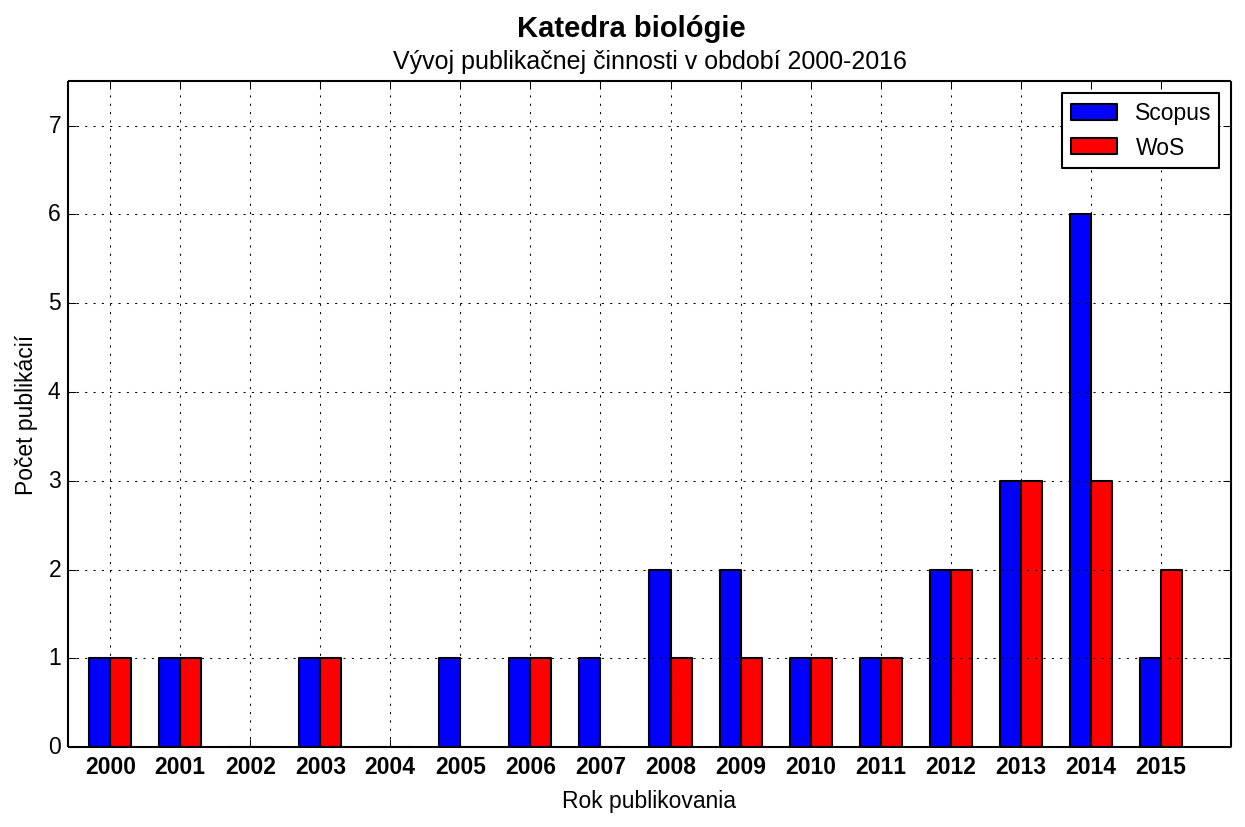
\includegraphics[width=\textwidth]{obr/plot-bio-publications.png}
  \caption{Vývoj publikačnej činnosti pracovníkov Katedry biológie v~období 2000--2016.}
  \label{fig:plot.bio.publications}
\end{figure}

Citovanosť článkov pracovníkov Katedry biológie podľa roku ich publikovania
zobrazuje graf na obr.\,\ref{fig:plot.bio.citations}.  Krivky dát zo Scopusu a
WoS sú takmer podobné, s~výnimkou už spomenutého \uv{chýbajúceho} roku 2005.

\begin{figure}
  \centering
  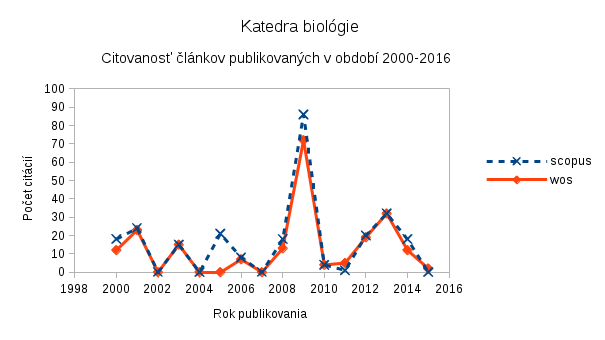
\includegraphics[width=\textwidth]{obr/plot-bio-citations.png}
  \caption{Citovanosť článkov pracovníkov Katedry biológie za obdobie 2000--2016.}
  \label{fig:plot.bio.citations}
\end{figure}


\section{Vývoj publikačnej činnosti a citovanosti pracovníkov Katedry biotechnológií v~čase}

Na grafe (obr.\,\ref{fig:plot.biotech.publications}) vidíme rozdiel medzi dátami
zo Scopusu a WoS.  Zdôrazníme 2 záznamy z~roku 2001, ktoré nie sú v~zozname zo
Scopusu Sú veľmi dobre citované ako ukazuje začiatok krivky WoS na obrázku
\ref{fig:plot.biotech.citations}.  Prekvapujúci je vyšší počet článkov obdobi
2010--2011 v~prospech WoS je spôsobený troma príspevkami do \emph{Proceedings of
  The 6\textsuperscript{th} International Conference on
  Polysaccharides-Glycoscience} a dvoma článkami z~\emph{Current Opinion in
  Biotechnology}, ktoré nie sú v~dátach zo Scopusu.  Relatívne minimum v~počtu
publikácií z~roku 2012 na rozdiel od celkových dát
(obr.\,\ref{fig:plot.fns.publications}) pre WoS tvorí už spomenutých 16 kapitol
knihy \emph{Handbook of Magentochemical Formulae} doc.\,Boču z~Katedry chémie.

\begin{figure}
  \centering
  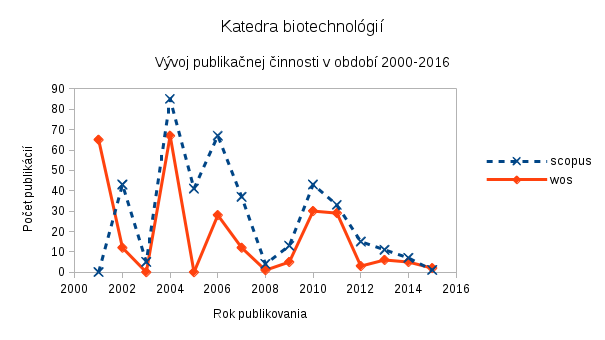
\includegraphics[width=\textwidth]{obr/plot-biotech-publications.png}
  \caption{Vývoj publikačnej činnosti pracovníkov Katedry biotechnológií v~období 2000--2016.}
  \label{fig:plot.biotech.publications}
\end{figure}

Prvú vec, ktorú si môžeme všimnúť na obrázku~\ref{fig:plot.biotech.citations} je
extrémne veľká citovanosť (65 citácií) 15 rokov starých článkov, ktoré nie sú
zahrnuté v~dátach zo Scopusu.  Naopak jeden dokument s~29 citáciami z~roku 2002
nie je v~dátach zo WoS a druhý má menej citácií v~WoS.  Podobne ako dokumenty
z~roku 2006 (článok s~32 citáciami nie je v~dátach WoS).  Inak citačné pokrytie
WoS kopíruje trend dát zo Scopusu.

\begin{figure}
  \centering
  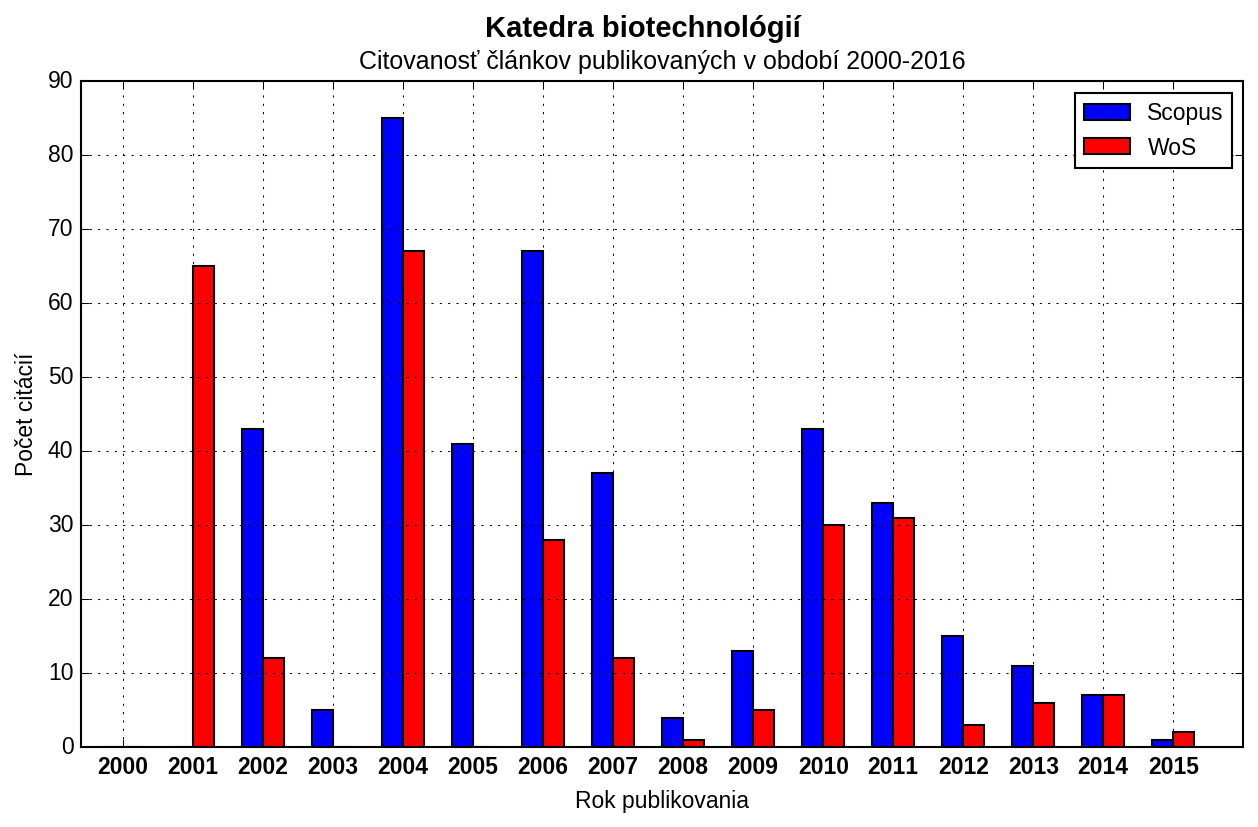
\includegraphics[width=\textwidth]{obr/plot-biotech-citations.png}
  \caption{Citovanosť článkov pracovníkov Katedry biotechnológií za obdobie 2000--2016.}
  \label{fig:plot.biotech.citations}
\end{figure}


\section{Vývoj publikačnej činnosti a citovanosti pracovníkov Katedry chémie
v~čase}

Publikácie Katedry chémie tvoria väčšinu získaných citačných záznamov (54\,\%
pre Scopus a 59\,\% pre WoS).  Z~toho dôvodu grafické zobrazenie počtu článkov
v~rokoch ich publikácie (obr.\,\ref{fig:plot.chem.publications}) je veľmi podobné
ku grafu počtu publikácii celej fakulty (obr.\,\ref{fig:plot.fns.publications}).

\begin{figure}
  \centering
  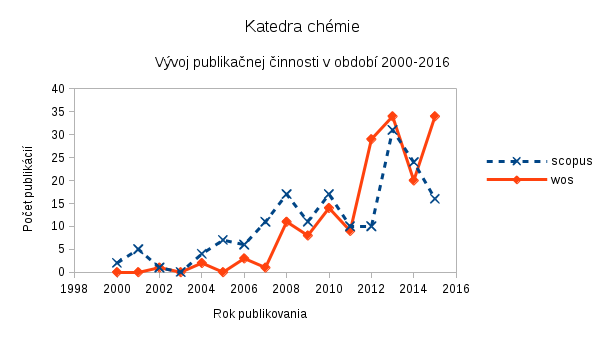
\includegraphics[width=\textwidth]{obr/plot-chem-publications.png}
  \caption{Vývoj publikačnej činnosti pracovníkov Katedry chémie v~období 2000--2016.}
  \label{fig:plot.chem.publications}
\end{figure}

Pretože publikácie Katedry chémie tvoria viac než polovicu záznamov dát graf
citácií (obr.\,\ref{fig:plot.chem.citations}) je veľmi podobný než publikácií
celej katedry (obr.\,\ref{fig:plot.fns.citations}).  Hlavným rozdielom absencia
záznamov z~WoS v~rokoch 2000--2001 a suma citácií článkov z~roku 2010 je
podstate rovnaká pre záznamy z~WoS a Scopusu.

\begin{figure}
  \centering
  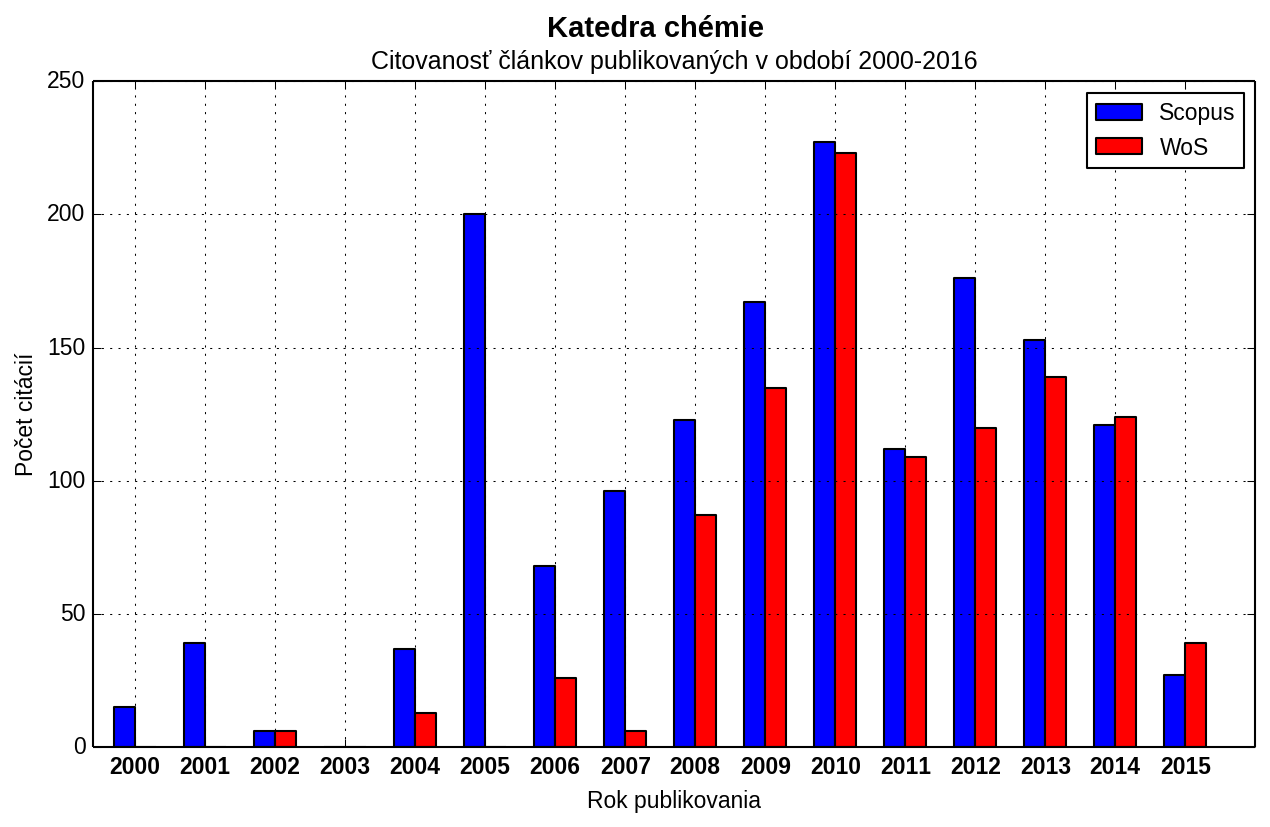
\includegraphics[width=\textwidth]{obr/plot-chem-citations.png}
  \caption{Citovanosť článkov pracovníkov Katedry chémie za obdobie 2000--2016.}
  \label{fig:plot.chem.citations}
\end{figure}


\section{Vývoj publikačnej činnosti a citovanosti pracovníkov Katedry ekochémie
  a rádioekológie v~čase}

V~grafickom zobrazení článkov podľa roku publikácie pracovníkov Katedry
ekochémie a rádiobiológie (obr.\,\ref{fig:plot.eco.publications}) môžeme vidieť
prepad publikačnej činnosti v~období 2007--2012.  V~roku 2009 nebola publikovaná
ani jedna práca resp. v~dátach chýba.  Pravdepodobne tento fenomén súvisí zo
založením Katedry ekochémie a rádiobiológie v~tomto období.  Vidíme typickú
absenciu dát z~WoS pre rok 2005 a nižší počet publikácií v~rokoch 2007 a 2014 na
rozdiel od dáť zo Scopusu.

\begin{figure}
  \centering
  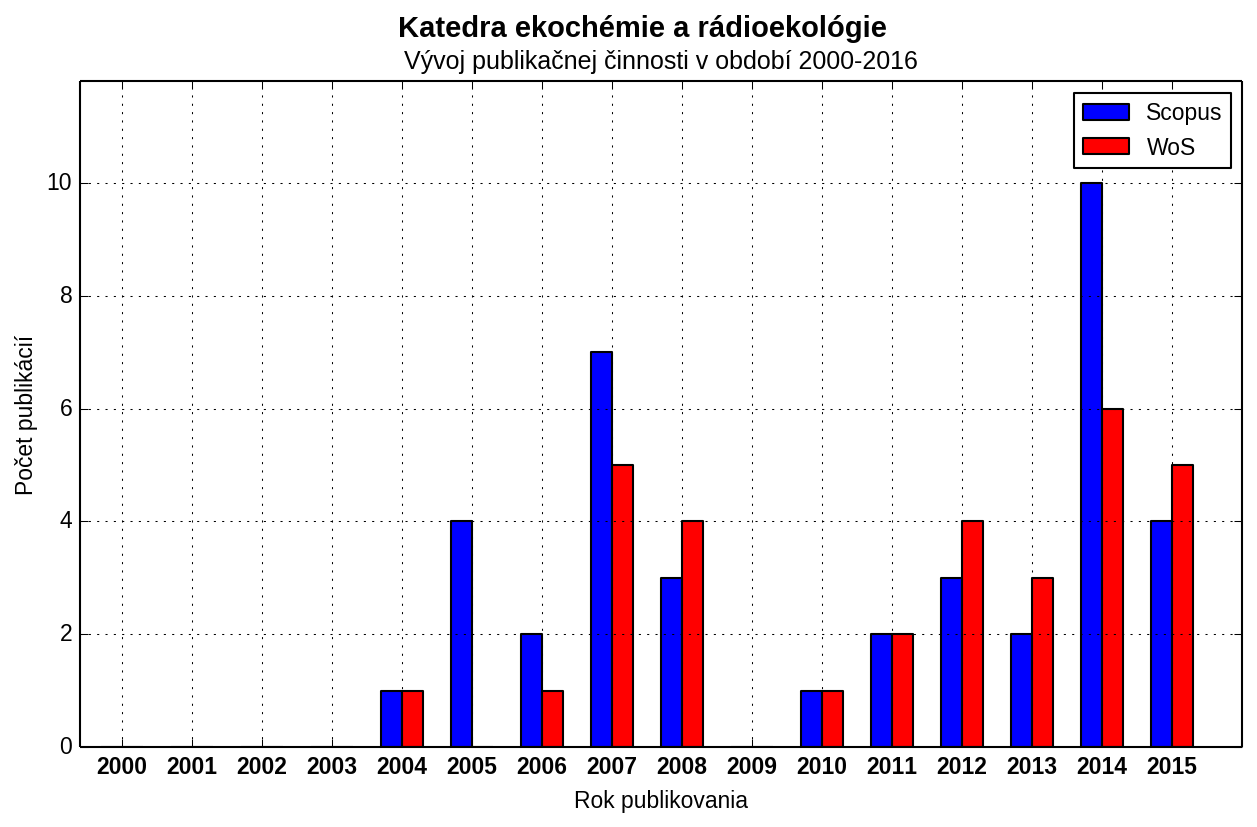
\includegraphics[width=\textwidth]{obr/plot-eco-publications.png}
  \caption{Vývoj publikačnej činnosti  pracovníkov Katedry ekochémie v~období 2000--2016.}
  \label{fig:plot.eco.publications}
\end{figure}

Citácie na články publikované pracovníkmi Katedry ekochéme a rádioekológie
zobrazuje obr.\,\ref{fig:plot.eco.citations}.  Je pozoruhodné, že od roku 2008
krivky počtu citácií pre WoS a Scopus takmer kopírujú rovnaký trend napriek
rozdieloch v~počtu záznamov pre roky 2012 až 2014 (hlavne pre rok 2014).  To
znamená, že dáta publikácií pracovníkov Katedry ekochémie z~WoS a Scopusu sú
presné okrem už spomínaného roku 2005.

\begin{figure}
  \centering
  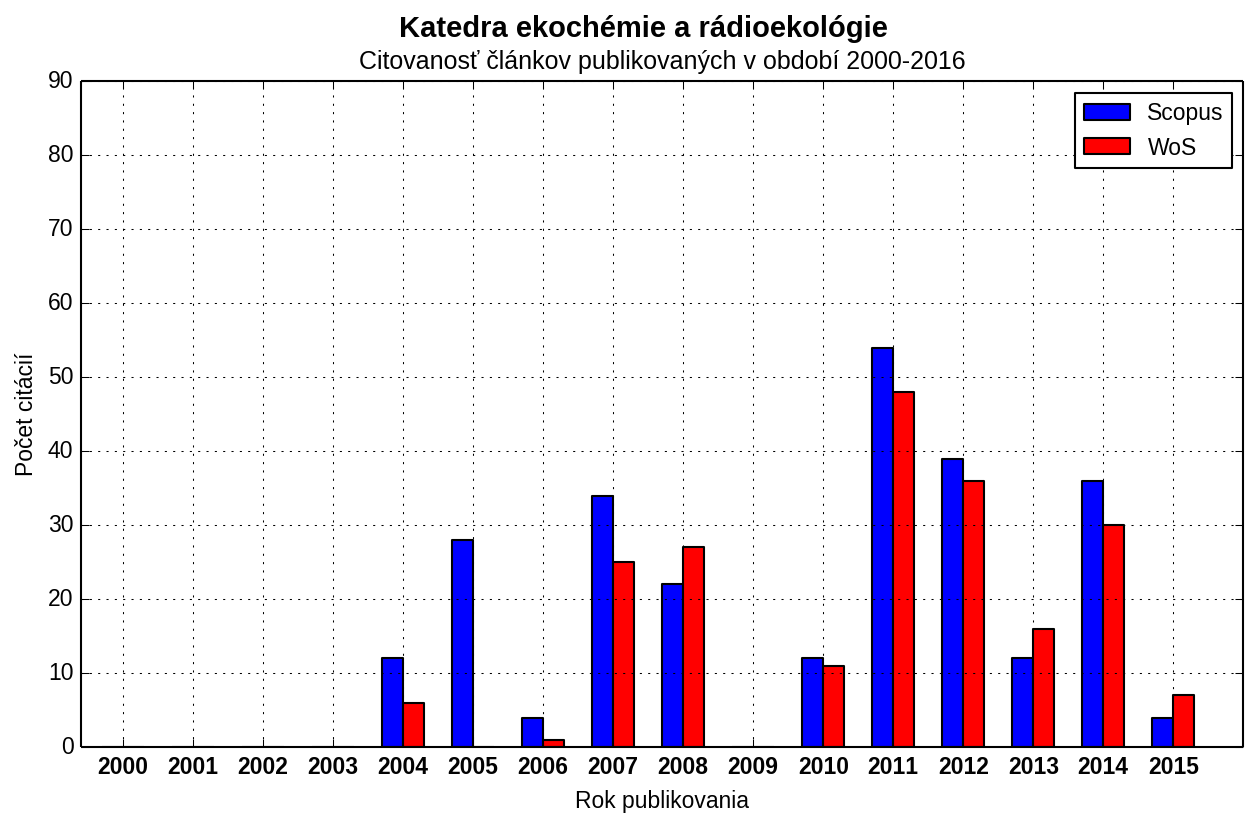
\includegraphics[width=\textwidth]{obr/plot-eco-citations.png}
  \caption{Citovanosť článkov pracovníkov Katedry ekochémie a rádioekológie za obdobie 2000--2016.}
  \label{fig:plot.eco.citations}
\end{figure}


\section{Vývoj publikačnej činnosti a citovanosti pracovníkov Katedry aplikovanej informatiky a matematiky v~čase}

Obrázok~\ref{fig:plot.inf.publications} je typickým príkladom, že z~malého
množstva dát nie je možné nič odvodzovať.  Keďže z~citačného registru WoS sa nám
podarilo získať iba 6 záznamov s~jednou citáciou (článok z~roku 2014) lepšie je
tieto dáta vôbec nepoužiť v~citačnej analýze.  Zaujímavé je, že z~roku nemáme
ani jednu publikáciu, rovnako ako v~prípade dát Katedry ekochémie.  Môže to
vypovedať o~podstatnejším zmenách na pôde Fakulty prírodných vied v~roku 2009.

\begin{figure}
  \centering
  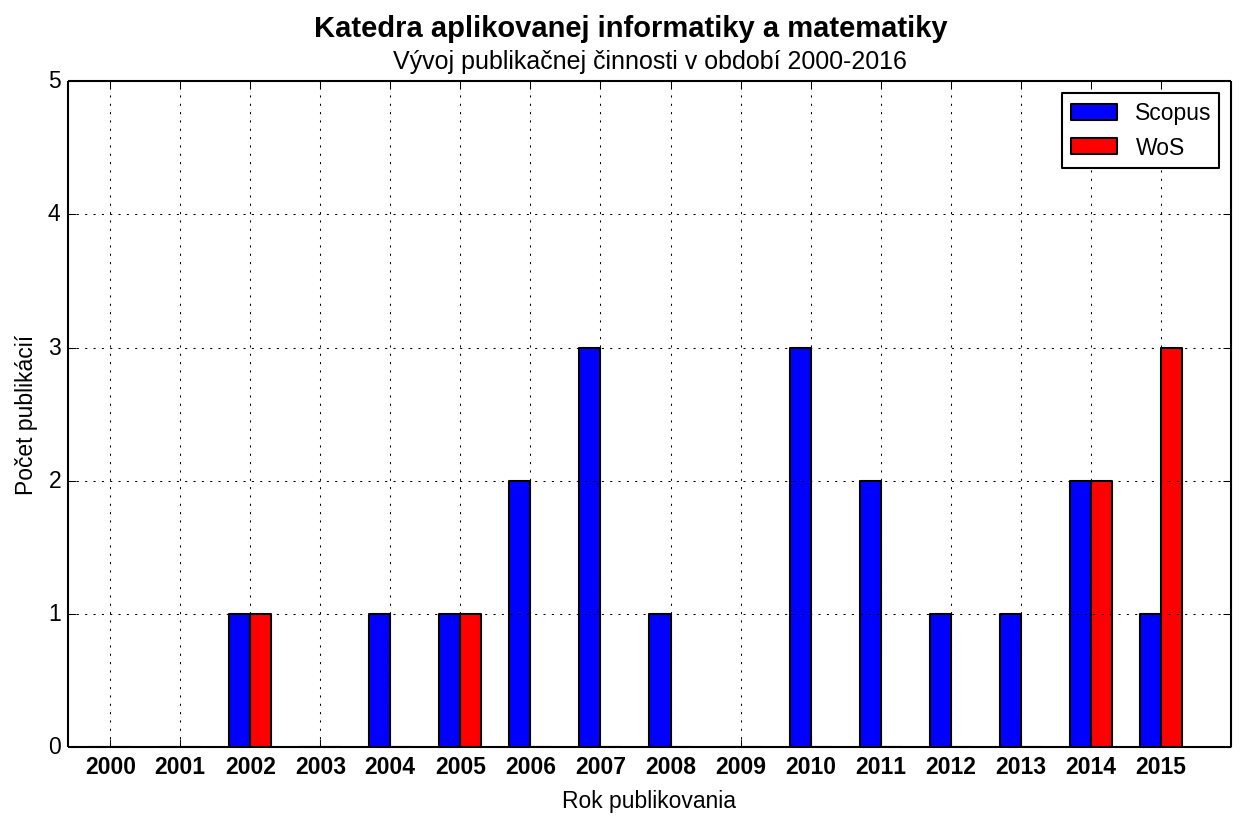
\includegraphics[width=\textwidth]{obr/plot-inf-publications.png}
  \caption{Vývoj publikačnej činnosti pracovníkov Katedry aplikovanej
    informatiky a matematiky v~období 2000-2016.}
  \label{fig:plot.inf.publications}
\end{figure}

\begin{figure}
  \centering
  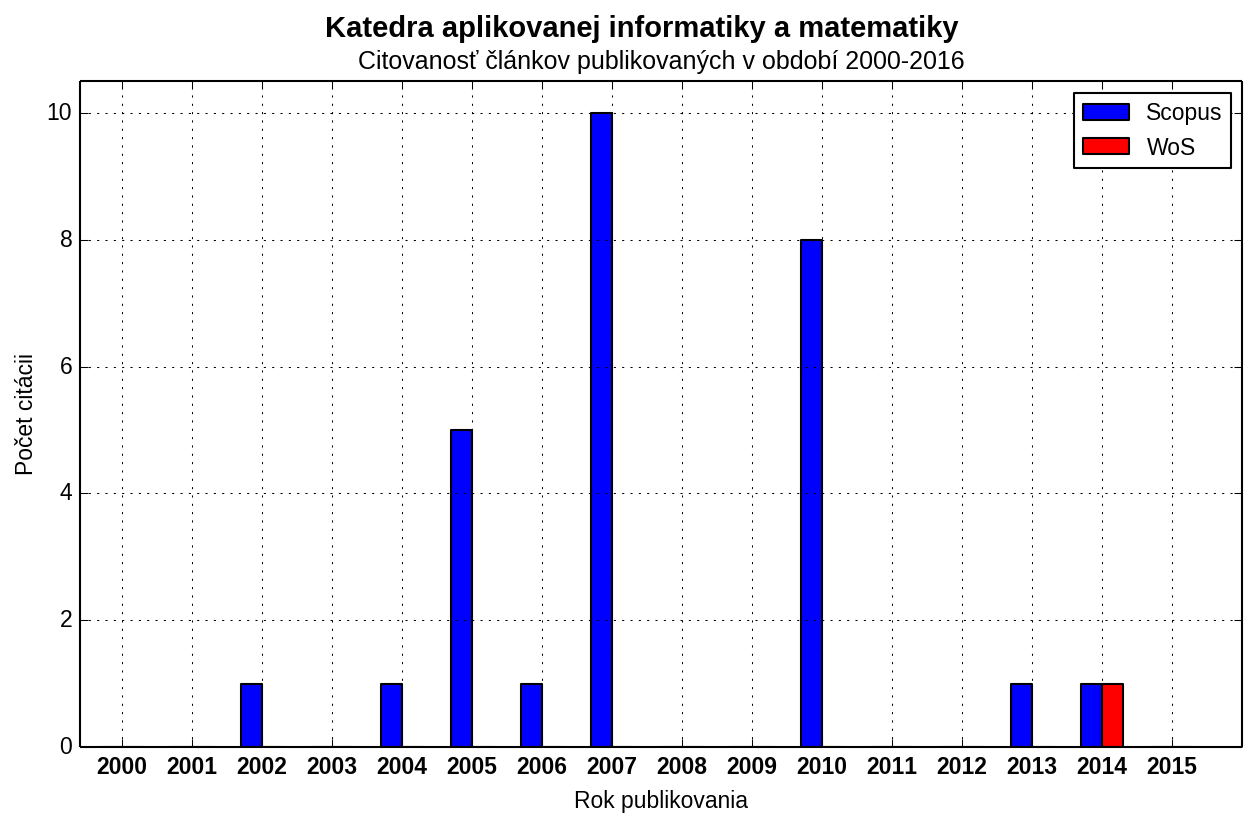
\includegraphics[width=\textwidth]{obr/plot-inf-citations.png}
  \caption{Citovanosť článkov pracovníkov Katedry aplikovanej informatiky a
    matematiky za obdobie 2000-2016.}
  \label{fig:plot.inf.citations}
\end{figure}


\section{Scientometrická analýza publikačnej činnosti katedier FPM UCM z~citačných registrov WoS a Scopus pomocou programu PoP}

Súbory dát pre jednotlivé katedry sme spracovali v~programe
PoP\footnote{\url{http://www.harzing.com/resources/publish-or-perish}}.  Výstup
programu v~20 stĺpcoch sme rozdelili do štyroch tabuliek
(tab.\,\ref{tab:citation.info} a tab.\,\ref{tab:citation.info2} pre základné
citačné údaje; tab.\,\ref{tab:citation.indicators} a
tab.\,\ref{tab:citation.indicators2} pre citačné indikátory).  Druhý a tretí
stĺpec tabuľky~\ref{tab:citation.info} predstavujú celkový počet publikácií a
celkový počet citácií, základné údaje pre citačnú analýzu (napr. výpočet impakt
faktoru).  Najväčší počet článkov tvorí blok Katedry chémie (54\,\% pre Scopus a
59\,\% pre WoS z~celej fakulty) a pochopiteľne najväčšiu časť citácií (62\,\%
pre Scopus a 60\,\% pre WoS z~celej fakulty).  Vek v~rokoch znamená koľko rokov
ubehlo od publikácie najstaršieho článku (12 v~prípade Katedry ekochémie
znamená, že prvé publikácie sú z~roku 2004).

Priemerný počet citácií na počet článkov (v~tab.\,\ref{tab:citation.info}
nazvaný Citácie/článok) je jednoduchý podiel celového počtu citácií počtom
článkov.  Podobný je priemerný počet citácií na rok (Citácie/rok), ktorý sa
vypočíta ako podiel citácií/článok a veku v~rokoch.  Citácie/autor získame
spočítaním podielov počtu citácií na článok počtom jeho autorov pre každý
článok.  Články/autor sa vypočíta sčítaním čiatkových hodnôt (1/počet autorov
daného článku) pre každý článok.  Priemerný počet autorov na článok
(Autori/článok) je jednoduchý podiel počtu všetkých autorov počtom článkov
(Harzling, 2010).

Hlavnou nevýhodou týchto základných metrík je veľká citlivosť na krajné hodnoty.
Môžeme to vidieť na porovnaní dát tých istých ľudí z~registrov Web of Science a
scopus.  Napr. priemerný počet citácií na počet článkov sa zhoduje iba v~prípade
dát Katedry ekochémie (6,27) a všetkých ostatných prípadoch sú hodnoty veľmi
odlišné.  Toto platí takmer pre všetky základné metriky.  Okrem priemerného
počtu autorov na článok, pri ktorom hodnoty varírujú medzi 4 a 5 (s~výnimkou dát
Katedry aplikovanej informatiky).

Citačné indikátory v~tabuľkách~\ref{tab:citation.indicators} a
\ref{tab:citation.indicators2} sú rozobrané v~kapitole
\ref{sec:citation.indicators} (s~výnimkou citácie/autori/rok a pokrytia $h$ a
$g$ indexov).  Priemerný počet citácií na autora a rok je podiel citácie/autor
celkovým vekom dát.  Pokrytie $h$ a $g$ indexov predstavuje percenuálny podiel
citácií použitých na výpočet $h$ a $g$ indexu.

Katedra chémie UCM dosahuje úroveň $h$-indexu katedry chémie na Univezite na Kréte
(LAZARIDIS, 2010).

\begin{table}
\centering\small
\begin{tabular}{llccccc}
  \hline\noalign{\vspace{.3ex}}
  Dátový súbor & Citačný  & Počet   & Počet   & Vek      & Citácie/ & Citácie/ \\
               & register & článkov & citácii & v~rokoch & rok      & článok   \\[0.3ex]
  \hline\noalign{\vspace{.5ex}}
  Celá fakulta   & Scopus & 324 & 2\:524 & 16 & 157,75 & 7,79 \\
                 & WoS    & 288 & 1\:712 & 16 & 107,00 & 5,94 \\[1ex]
  Biológia       & Scopus &  28 &    265 & 16 &  16,56 & 9,46 \\
                 & WoS    &  26 &    219 & 16 &  13,56 & 8,42 \\[1ex]
  Biotechnológie & Scopus &  67 &    406 & 15 &  27,07 & 6,01 \\
                 & WoS    &  58 &    267 & 15 &  17,80 & 4,60 \\[1ex]
  Chémia         & Scopus & 175 & 1\:567 & 16 &  97,94 & 8,95 \\
                 & WoS    & 170 & 1\:026 & 14 &  73,29 & 6,04 \\[1ex]
  Ekochémia      & Scopus &  41 &    257 & 12 &  21,42 & 6,27 \\
                 & WoS    &  33 &    207 & 12 &  17,25 & 6,27 \\[1ex]
  Informatika    & Scopus &  18 &     28 & 14 &   2,00 & 1,56 \\
                 & WoS    &  -- &     -- & -- &  --    & --   \\[0.5ex]
  \hline
\end{tabular}
\caption{Základné citačné informácie.}
\label{tab:citation.info}
\end{table}


\begin{table}
\centering\small
\begin{tabular}{llccc}
  \hline\noalign{\vspace{.3ex}}
  Dátový súbor & Citačný  & Citácie/ & Články/ & Autori/ \\
               & register & autor    & autor   & článok  \\[0.3ex]
  \hline\noalign{\vspace{.5ex}}
  Celá fakulta   & Scopus & 662,43 & 83,89 & 4,78 \\
                 & WoS    & 425,01 & 84,58 & 4,70 \\[1ex]
  Biológia       & Scopus &  88,59 &  9,23 & 3,93 \\
                 & WoS    &  56,53 &  7,10 & 4,19 \\[1ex]
  Biotechnológie & Scopus &  93,43 & 16,32 & 4,79 \\
                 & WoS    &  64,51 & 14,33 & 4,90 \\[1ex]
  Chémia         & Scopus & 405,62 & 41,56 & 5,06 \\
                 & WoS    & 256,15 & 54,63 & 4,72 \\[1ex]
  Ekochémia      & Scopus &  62,12 &  9,97 & 4,85 \\
                 & WoS    &  48,45 &  7,77 & 4,97 \\[1ex]
  Informatika    & Scopus &  11,67 &  7,95 & 2,78 \\
                 & WoS    &  --    & --    & --   \\[0.5ex]
  \hline
\end{tabular}
\caption{Pokračovanie základných citačných informácii.}
\label{tab:citation.info2}
\end{table}

\begin{table}
\centering\small
\begin{tabular}{llcccccccc}
  \hline\noalign{\vspace{.3ex}}
  Dátový súbor & Citačný  & $h$ & $g$ & $h^{\mathrm{c}}$ & $h_{\mathrm{I}}$ & $h_{\mathrm{I, norm}}$ & AWCR & AW    & AWCR/ \\
               & register &     &     &                  &                  &                        &       & index & autor \\[0.3ex]
  \hline\noalign{\vspace{.5ex}}
  Celá fakulta   & Scopus & 26 & 36 & 21 & 4,76 & 12 & 488,95 & 22,11 & 127,24 \\
                 & WoS    & 22 & 31 & 20 & 4,44 & 10 & 400,05 & 20,00 &  95,77 \\[1ex]
  Biológia       & Scopus & 10 & 16 &  8 & 2,44 &  6 &  46,66 &  6,83 &  13,00 \\
                 & WoS    &  8 & 14 &  7 & 1,68 &  4 &  42,63 &  6,53 &  10,13 \\[1ex]
  Biotechnológie & Scopus & 10 & 18 &  8 & 1,96 &  5 &  52,12 &  7,36 &  12,16 \\
                 & WoS    &  7 & 15 &  5 & 1,63 &  5 &  34,80 &  5,90 &   7,68 \\[1ex]
  Chémia         & Scopus & 22 & 32 & 18 & 4,07 & 10 & 324,90 & 18,02 &  84,17 \\
                 & WoS    & 17 & 26 & 16 & 3,36 &  7 & 270,74 & 16,45 &  64,02 \\[1ex]
  Ekochémia      & Scopus &  9 & 13 &  8 & 1,88 &  4 &  59,02 &  7,68 &  16,23 \\
                 & WoS    &  8 & 12 &  8 & 1,64 &  4 &  54,52 &  7,38 &  14,15 \\[1ex]
  Informatika    & Scopus &  3 &  4 &  2 & 1,00 &  2 &   3,99 &  2,00 &   1,61 \\
                 & WoS    & -- & -- & -- &  --  & -- &  --    & --    &  --    \\[0.5ex]
  \hline
\end{tabular}
\caption{Citačné indikátory.}
\label{tab:citation.indicators}
\end{table}

\begin{table}
\centering\small
\begin{tabular}{llccccc}
  \hline\noalign{\vspace{.3ex}}
  Dátový súbor & Citačný  & $e$ & $h_{\mathrm{m}}$ & Citácia/   & Pokrytie        & Pokrytie        \\
               & register &     &                  & autora/rok & $h$-indexu (\%) & $g$-indexu (\%) \\[0.3ex]
  \hline\noalign{\vspace{.5ex}}
  Celá fakulta   & Scopus & 20,62 & 13,62 & 41,40 & 44 & 53 \\
                 & WoS    & 18,71 & 10,67 & 26,56 & 49 & 58 \\[1ex]
  Biológia       & Scopus & 10,86 &  4,94 &  5,53 & 82 & 97 \\
                 & WoS    & 10,39 &  3,64 &  3,50 & 79 & 95 \\[1ex]
  Biotechnológie & Scopus & 13,75 &  4,84 &  6,67 & 72 & 87 \\
                 & WoS    & 13,08 &  3,18 &  4,30 & 82 & 93 \\[1ex]
  Chémia         & Scopus & 19,65 & 10,01 & 25,35 & 56 & 67 \\
                 & WoS    & 16,49 &  8,00 & 18,29 & 55 & 66 \\[1ex]
  Ekochémia      & Scopus &  8,60 &  4,90 &  5,17 & 60 & 73 \\
                 & WoS    &  8,12 &  4,18 &  4,03 & 63 & 76 \\[1ex]
  Informatika    & Scopus &  3,32 &  1,42 &  0,83 & 71 & 82 \\
                 & WoS    & --    & --    & --    & -- & -- \\[0.5ex]
  \hline
\end{tabular}
\caption{Pokračovanie citačných indikátorov.}
\label{tab:citation.indicators2}
\end{table}


%%% Local Variables:
%%% TeX-master: "diplomovka"
%%% End: